\chapter{Heuristics}
\lecture{5}{4/11}

\begin{example}
    Following are some example heuristics that may be used to solve the travelling salesman problem:
    \begin{enumerate}
        \item the distance to the nearest unvisited city;
        \item the shortest path of length $k$ through unvisited cities;
        \item the distance of greedy completion;
        \item the distance of any partial completion through unvisited cities;
        \item the distance of partial tour formed by inserting a city; and
        \item the distance of the partial tour formed by inserting a path.
    \end{enumerate}
\end{example}

\begin{definition}[Admissable]
    We say that a heuristic is \textbf{admissable} if it never overestimates.
\end{definition}

\begin{problem}[8-puzzle problem]
    Our state space for this problem is $S = M_3(\{0, 1, \ldots, 8\})$ where if $s \in S$ then $s_{ij} \neq s_{kl}$ for all $(i,j) \neq (k, l)$. Let $s \in S$. Then $s' \in S$ iff all the elements are the same except the $0$ element has been swapped with a horizontally or vertically adjacent element. Our initial and goal state are arbitrary and the step cost is constant for each transititon. 
\end{problem}

\begin{example}[Heuristics for the 8-puzzle problem]
    Consider the 8-puzzle problem formally defined above. An uninformed search generates large searchg trees, so it is appropriate that we find a good heuristic. Some common heuristics:
    \begin{enumerate}
        \item number of misplaced tiles in a state ($h_1$); and
        \item the sum of the distances each tile is from their goal position assuming an empty grid (Manhattan distance) ($h_2$).
    \end{enumerate}
    Both of these heuristics are admissable. Experimental evidence suggests that $h_2$ is a beter heuristic. In fact, $h_2$ is always better than $h_1$, but what do we mean by \emph{better}.
\end{example}

\begin{figure}
    \centering
    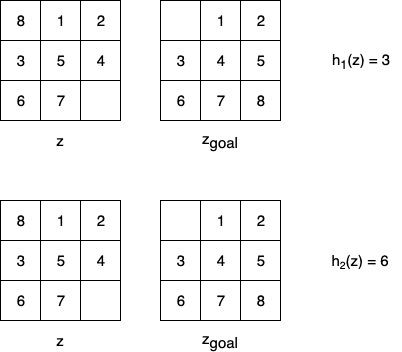
\includegraphics[width=0.6\linewidth]{images/8-puzzle-ex-1.png}
    \caption{$8$-puzzle example heuristics.}
\end{figure}

\begin{definition}[Domination]
    Let $h_1, h_2$ be two heuristic functions. We say that $h_2$ \textbf{dominates} $h_1$ if $h_2(z) \geq h_1(z)$ for all $z$.
\end{definition}

\begin{theorem}[]
    Let $h$ be an admissable heuristic and $s(z_1, z_2)$ be a step cost function such that there exists a $\varepsilon > 0$ such that $s > \varepsilon$. Also let the branching factor be bounded by $b$. Then A* search will expand all nodes for which $f(z) < c^\star$ where $c^\star$ is the optimal path cost to a goal node.
\end{theorem}

\begin{remark}
    This is a clear observation, but if two heuristic functions are admissable it is \emph{always} best to use the one with a higher value.
\end{remark}

To solve a problem, we can use heuristics that act as accurate approximations for simplified versions of the problem.

\begin{definition}[Subproblem]
    A \textbf{subproblem} is a (typically) smaller problem that is first solved in order to solve a different problem.
\end{definition}

This is a relatively wavey definition, but we can define a certain type of subproblem.

\begin{definition}[Relaxed problem]
    A problem with fewer restrictions on the actions is called a \textbf{relaxed problem}.
\end{definition}

The cost on an optimal solution in a relaxed problem is an admissable heuristic for the original problem. \emph{This is an important concept.}

Additionally, any solution to a problem is also a solution to a relaxed problem, but it may not be optimal. So to find a heuristic for a problem, we can solve the relaxed problem.

If we have a problem defined in formal language, we can generate heuristics by looking at the subproblems geneerated by removing conditions.

\begin{example}[Subproblem heuristic for the $8$-puzzle problem]
    Above we defined the problem as \emph{a tile can move from cell $A$ to cell $B$ if cell $A$ is horizontally or vertically adjacent to $B$ and $B$ is blank}. Here we can remove one or both of the two requirements to genereate 3 subproblems, that is:
    \begin{enumerate}
        \item \emph{a tile can move from cell $A$ to cell $B$ if cell $B$ is blank};
        \item \emph{a tile can move from cell $A$ to cell $B$ if $A$ is horizontally or vertically adjacent to $B$}; and
        \item \emph{a tile can move from cell $A$ to cell $B$}.
    \end{enumerate}
\end{example}

For heuristics for subproblems to be practical, they must be efficiency solvable.

\begin{proposition}
    Now let's consider a situation where we are given many admissable heuristic functions $h_1, h_2, \ldots, h_n$ but none of them dominate each other. We can define another admissable heuristic function that \emph{dominates} $h_1, h_2, \ldots, h_n$ as
    \[ h(z) = \max_{i \in \{1, 2, \ldots, n\}}{(h_i)}. \]
\end{proposition}

\begin{proof}
    It is clear to see that $h$ is also admissable, as if $h_1, h_2, \ldots, h_n$ never overestimate then the maximum of these values also does not overestimate. Again, it is clear to see that $h$ dominates $h_1, h_2, \ldots, h_n$ as for all $h_i$, $h \geq h_i$.
\end{proof}
